% POLIMI beamer template
%
% authors: Davide Tateo, Stefano Paladino 
% 19-09-2014
%

\documentclass{beamer}
\usepackage{animate}
\usepackage[utf8]{inputenc}
\usepackage{wrapfig}
%\usepackage{lmodern}
\usepackage{enumerate}
\usepackage{multimedia}
\usepackage[skip=0pt]{subcaption}
\usepackage{xspace}
\usepackage{xmpmulti}
\usepackage{tabularx}
\usepackage{tabto}
\usepackage{media9}
\usepackage{array}
\usepackage{multicol}
\usepackage{afterpage}
\usepackage{amsmath,amssymb}            
\usepackage{rotating}  
\usepackage{fancyhdr}  
%\usepackage[scriptsize]{caption} 
\usepackage{cite}
\usepackage{hyperref}
\usepackage{amsthm}
\usepackage{xargs}

\usepackage{units}
%\usepackage{wrapfig}
\usepackage{cutwin}
\usepackage[calc]{adjustbox}
\usepackage{booktabs}
\usepackage{mathtools}
\usepackage[makeroom]{cancel}
\usepackage{caption, subcaption}
\usepackage{xcolor}
\usepackage{graphicx,array}

\usepackage{algorithm}
\usepackage{algorithmicx}
\usepackage{algpseudocode}


\newcolumntype{C}[1]{>{\centering\let\newline\\\arraybackslash\hspace{0pt}}m{#1}}
\newcolumntype{L}[1]{>{\raggedright\let\newline\\\arraybackslash\hspace{0pt}}m{#1}}

\renewcommand{\arraystretch}{1.2}% Spread rows out...
\newcolumntype{O}[1]{>{\centering}m{#1}} 

\newcommand{\norm}[2][1]{\left\| #2 \right\|_{#1}}

\newcommand{\vtheta}{{\boldsymbol{\theta}}}
\newcommand{\de}{\, \textrm{d}}
\newcommand{\sspace}{\mathcal{S}}
\newcommand{\aspace}{\mathcal{A}}
\newcommand{\tfunc}{\mathcal{P}}
\newcommand{\rfunc}{\mathcal{R}}
\newcommand*{\gradj}{\nabla_{\vtheta}J(\vtheta)}

\DeclareRobustCommand{\eg}{e.g.,\@\xspace}
\DeclareRobustCommand{\ie}{i.e.,\@\xspace}
\DeclareRobustCommand{\wrt}{w.r.t.\@\xspace}

\newcommand{\EVV}[2][\ppvect \in \ppspace]{\EV_{#1}\left[{#2}\right]}
%\newcommand{\norm}[2][\infty]{\left\|#2\right\|_{#1}}
\newcommand{\vphi}{\boldsymbol{\phi}}
\newcommand{\vv}{\boldsymbol{v}}
\newcommand{\vw}{\boldsymbol{w}}
\newcommand{\jbase}[1][t]{{J_{B}^{#1}}}
%\newcommand{\vtarget}[1][t]{{\underline{\vtheta}^{\,#1}}}
\newcommand{\vtarget}[1][t]{{\vtheta}^{#1}_T}
%\newcommand{\wtarget}[1][t]{{\underline{w}^{\,#1}}}
\newcommand{\wtarget}[1][t]{{{w_T}^{#1}}}
%\newcommand{\vtarget}[1][t]{{\vtheta_{target}^{#1}}}

\newcommand{\Aspace}{\mathcal{A}}
\newcommand{\Sspace}{\mathcal{S}}
\newcommand{\Tspace}{\mathcal{T}}
\newcommand{\Transition}{\mathcal{P}}
\newcommand{\Reward}{\mathcal{R}}
\newcommand{\policy}{\pi_{\vtheta}(a \vert s)}
%\newcommand{\pol}{\pi_{\vtheta}}
\newcommand{\gradJ}[2][\vtheta]{\nabla_{#1} J(#2)}
\newcommand{\score}[2]{\nabla_{\vtheta}\log p_{#1}(#2)}
\newcommand{\gradApp}[3][N]{\widehat{\nabla}_{#2}^{#1}J(#3)}
%\newcommand{\Deltav}{\underline{\Delta_{\vv}}J}
\newcommand{\Deltav}{\mathcal{L}}
\newcommand{\gradDelta}[1][w]{\nabla_{#1}\Deltav}
%\newcommand{\we}[1][]{{e^{#1w}}}
\newcommand{\we}[1][]{{\sigma ^{#1}}}
\renewcommand{\score}[2][\vtheta]{\nabla_{#2}\log p_{#1}(\tau)}
\newcommand{\gradlogsumpi}[4]{\sum_{#1=#2}^{#3}\nabla_{#4}\log\pi_{#1}}

\makeatletter
\newcommand{\algcolor}[2]{%
	\hskip-\ALG@thistlm\colorbox{#1}{\parbox{\dimexpr\linewidth-2\fboxsep}{\hskip\ALG@thistlm\relax #2}}%
}
\makeatother
\definecolor{aliceblue}{rgb}{0.94, 0.97, 1.0}
\definecolor{bisque}{rgb}{1.0, 0.89, 0.77}
\definecolor{teagreen}{rgb}{0.82, 0.94, 0.75}

\usetheme{Madrid}

%Information to be included in the title page:

\def\supervisor#1{\gdef\insertsupervisor{#1}}
\def\departament#1{\gdef\insertdepartament{#1}}
\def\defensetext#1{\gdef\insertdefensetext{#1}}


\newcolumntype{R}[1]{>{\raggedleft\let\newline\\\arraybackslash\hspace{0pt}}m{#1}}

\newenvironment{tightcenter}{%
  \setlength\topsep{0pt}
  \setlength\parskip{0pt}
  \begin{center}
}{%
  \end{center}
}

%\defbeamertemplate*{title page}{mydefault}[1][]
%{
%  %\vbox{}
%    %\vspace*{-8ex}
%    {\begin{wrapfigure}{l}{0.2\textwidth}
%  \begin{center}
%    
\includegraphics[height=1.5cm]{pictures/newlogo}
%  \end{center}
%\end{wrapfigure}  
%\usebeamerfont{institute}\Large POLITECNICO DI MILANO \newline \small {{\large S}CHOOL OF {\large I}NDUSTRIAL AND {\large I}NFORMATION {\large E}NGINEERING}}
%    
%    \begin{beamercolorbox}[wd=\paperwidth,sep=8pt,left,#1]{institute}
%     {\usebeamercolor[fg]{titlegraphic}\raisebox{-.4\height}{
\includegraphics[height=1.5cm]{pictures/newlogo.png}}}\quad
%     {\usebeamerfont{institute}\Large POLITECNICO DI MILANO \newline \small {{\large S}CHOOL OF {\large I}NDUSTRIAL AND {\large I}NFORMATION {\large E}NGINEERING}}
%    \end{beamercolorbox}
%  \vfill
%  \begin{centering}
%    \begin{beamercolorbox}[sep=8pt,center,#1]{title}
%      \usebeamerfont{title}\inserttitle\par%
%    \end{beamercolorbox}%
%    \vskip1em\par
%    \begin{beamercolorbox}[sep=8pt,center,#1]{date}
%      \usebeamerfont{author}Supervisor: \insertsupervisor\par\medskip
%      \insertauthor
%    \end{beamercolorbox}
%  \end{centering}
%  \vfill
%    \begin{beamercolorbox}[sep=8pt,center,#1]{date}
%      \usebeamerfont{date}\insertdate
%    \end{beamercolorbox}
%}


\defbeamertemplate*{title page}{mydefault}[1][]{
    %\begin{tabular}[t]{@{}O{0.11\textwidth} | O{0.82\textwidth}@{}}
    \begin{tabular}[t]{@{} m{0.11\textwidth} @{} m{0.4em} @{} m{0.82\textwidth} @{}}
        
\includegraphics[width=\linewidth]{pictures/newlogo} && \centering \vspace{0.0cm} {\Large POLITECNICO DI MILANO} \newline \small {\large S}CHOOL OF {\large I}NDUSTRIAL AND {\large I}NFORMATION {\large E}NGINEERING
    \end{tabular}

\vspace{3em}

  \begin{centering}
    \begin{beamercolorbox}[sep=8pt,center,rounded=true,shadow=true,#1]{title}
      \usebeamerfont{title}\inserttitle\par%
    \end{beamercolorbox}%
  \end{centering}

\vspace{3em}

\begin{tabular}[b]{@{} >{\raggedright\arraybackslash}p{0.5\textwidth} @{}%
   >{\raggedleft\arraybackslash}p{0.5\textwidth} @{}%
  }
Supervisor: Prof. Marcello Restelli &  \\
Co-supervisor: Dott. Matteo Papini & \\
 \\
& Andrea Battistello, 873795
\end{tabular}

\vspace{1.4em}

\centering
%25/07/2018
July 25, 2018

}


\title[Balancing Safety and Exploration]{Balancing Safety and Exploration in Policy Gradient}
%\subtitle{}

\author[Andrea Battistello]{Andrea Battistello}
\institute[PoliMI]{Politecnico di Milano}
%\logo{
\includegraphics[height=1.0cm]{pictures/newlogo.png}}
 

%\supervisor{Supervisor}{Prof. Marcello Restelli}
\date[25/07/2018]{25 Luglio 2018}

\supervisor{Prof. Marcello Restelli}


\begin{document}

\frame{\titlepage}

%%%%%%%%%%%%%%%%%%%%%%%%%%%%%%%%%%%%%%%%%%%%%%%%%%%%%%%%%%%%%%%%%%%%%%%%%%%%%%%%%%%%%%%%%%%%%%%%%%%%%%%%%%%%%%%%%%%%

% make your choice
%\polimititlepage % no logo
%\polimititlepage[polimi]
%\polimititlepage[airlab]
%\polimititlepage[necst]

%\addtocounter{framenumber}{-3}


\begin{frame}
\frametitle{Contents}
\tableofcontents
\end{frame}


%%%%%%%%%%%%%%%%%%%%%%%%%%%%%%%%%%%%%%%%%%%%%%%%%%%%%%%%%%%%%%%%%%%%%%%%%%%%%%%%%%%%%%%%%%%%%%%%%%%%%%%%%%%%%%%%%%%%
\AtBeginSection[] {
\begin{frame}
\frametitle{Contents}
\tableofcontents[currentsection]
\end{frame}
}
%%%%%%%%%%%%%%%%%%%%%%%%%%%%%%%%%%%%%%%%%%%%%%%%%%%%%%%%%%%%%%%%%%%%%%%%%%%%%%%%%%%%%%%%%%%%%%%%%%%%%%%%%%%%%%%%%%%
\section{Reinforcement Learning}

\begin{frame}
\frametitle{Reinforcement Learning}

We learn from the \textbf{interaction} with the environment \\
For each step, the agent performs an action and receives an observation

\vfill

\centering
\includegraphics[width=\textwidth]{pictures/mdp_agent_environment}

\end{frame}

%\begin{frame}{Example: Mountain Car}
%  \animategraphics[autoplay,loop,controls,width=\linewidth]{120}{pictures/animation/mc-}{0}{107}
%\end{frame}

\begin{frame}{Example: Mountain Car}
\centering 

  \animategraphics[autoplay,loop,width=0.9\linewidth]{30}{pictures/mountain_car_animation3}{}{}
\end{frame}


\begin{frame}
\frametitle{Example: Mountain Car}
\begin{figure}[t]
\begin{subfigure}{0.49\textwidth}
\includegraphics[width=\textwidth]{pictures/mc2}
\end{subfigure}
\hfill
\begin{subfigure}{0.49\textwidth}
\includegraphics[width=\textwidth]{pictures/mc3}
\end{subfigure}
\end{figure}
\end{frame}


%%%%%%%%%%%%%%%%%%%%%%%%%%%%%%%%%%%%%%%%%%%%%%%%%%%%%%%%%%%%%%%%%%%%%%%%%%%%%%%%%%%%%%%%%%%%%%%%%%%%%%%%%%%%%%%%%%%%%%%%%%%%%%%%%%%%%%%%%%%%%%%%%%%%%%%%%%%%%%%%%%%%%%%%%%%%%%%%%%%%%%%%%%%%%%%%%%%%%%%%%


%\begin{frame}
%\frametitle{Processi decisionali di Markov}
%
%Un processo decisionale di Markov (MDP) è una tupla $\left\langle \mathcal{S}, \mathcal{A}, \mathcal{P}, \mathcal{R}, \gamma, \mu\right\rangle$ dove:
%\begin{itemize}
%\item $\mathcal{S}$ è l'insieme di stati che l'agente può osservare
%\item $\mathcal{A}$ è l'insieme di azioni che l'agente può compiere
%\item $\mathcal{P}(s,a, s')$ è la funzione di transizione
%\item $\mathcal{R}(s,a)$ è la funzione di rinforzo
%\item $\gamma$ è un fattore di sconto
%\item $\mu$ rappresenta lo stato iniziale
%\end{itemize}
%
%\end{frame}

%%%%%%%%%%%%%%%%%%%%%%%%%%%%%%%%%%%%%%%%%%%%%%%%%%%%%%%%%%%%%%%%%%%%%%%%%%%%%%%%%%%%%%%%%%%%%%%%%%%%%%%%%%%%%%%%%%%%%%%%%%%%%%%%%%%%%%%%%%%%%%%%%%%%%%%%%%%%%%%%%%%%%%%%%%%%%%%%%%%%%%%%%%%%%%%%%%%%%%%%%

%\begin{frame}
%\frametitle{Processi decisionali di Markov}
%
%\begin{figure}
%\begin{subfigure}[t]{0.495\textwidth}
%\includegraphics[width=\textwidth]{pictures/mdp_example}
%\caption{Rappresentazione di un MDP}
%\end{subfigure}
%\hfill
%\begin{subfigure}[t]{0.495\textwidth}
%\includegraphics[width=\textwidth]{pictures/mdp_policy}
%\caption{Rappresentazione di una politica}
%\end{subfigure}
%\end{figure}
%
%\end{frame}

%%%%%%%%%%%%%%%%%%%%%%%%%%%%%%%%%%%%%%%%%%%%%%%%%%%%%%%%%%%%%%%%%%%%%%%%%%%%%%%%%%%%%%%%%%%%%%%%%%%%%%%%%%%%%%%%%%%%%%%%%%%%%%%%%%%%%%%%%%%%%%%%%%%%%%%%%%%%%%%%%%%%%%%%%%%%%%%%%%%%%%%%%%%%%%%%%%%%%%%%%

\begin{frame}
\frametitle{A Reinforcement Learning method}
\begin{block}{Policy}
A policy $\pi_{\vtheta}$ is a function that maps states to actions
\end{block}

\begin{block}{Performance}
The performance $J(\vtheta)$ of a policy is the discounted sum of rewards obtained by following $\pi_{\vtheta}$
\[
J(\vtheta) = \sum_{k=0}^T \gamma^k r(s_k, a_k)
\]
\end{block}

\begin{block}{Policy Gradient method}
The optimal policy can be found by gradient ascent on policy parameters: 
\[
\vtheta \gets \vtheta + \alpha \gradj
\]
\end{block}

\end{frame}


\begin{frame}{Gaussian policies}

\begin{table}
\begin{tabular}[t]{m{0.4\textwidth}  m{0.6\textwidth}}

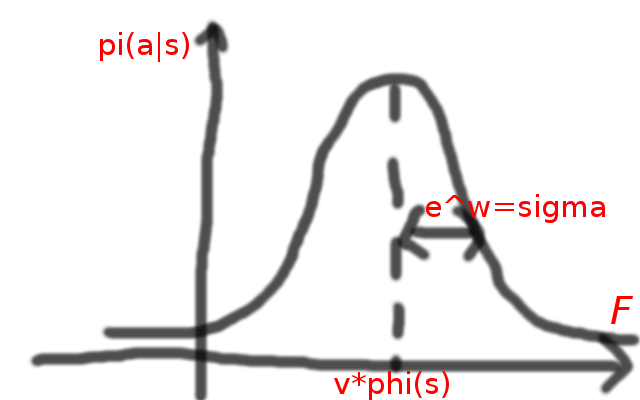
\includegraphics[width=0.4\textwidth]{pictures/gauss.png} &
\begin{minipage}{0.5\textwidth}\Large
\begin{align*}
s = [x; \dot{x}] \\ \vtheta = [\vv; w]
\end{align*}
\end{minipage}
 \\
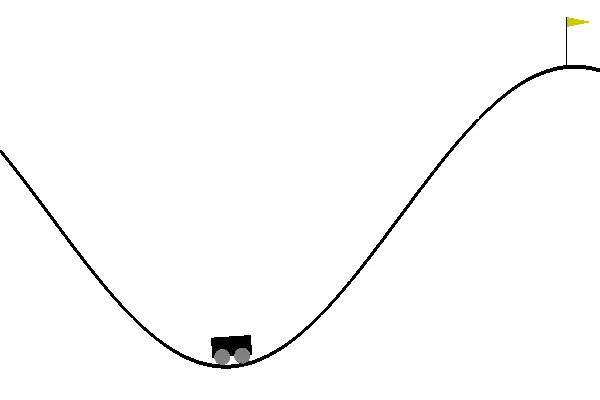
\includegraphics[width=0.4\textwidth]{pictures/mountain_car} &
 \begin{minipage}{0.5\textwidth}\Large \begin{equation*}
\pi(a|s) = \frac{1}{\sqrt{2\pi}\sigma}e^{-\frac{1}{2}\left(\frac{a - \vv\phi(s)}{\sigma}\right)^2}
\end{equation*}
\end{minipage}

\end{tabular}
\end{table}

\end{frame}


\section{Safe Reinforcement Learning}

\begin{frame}{Safe Reinforcement Learning}
\begin{figure}
\begin{subfigure}[t]{0.495\textwidth}
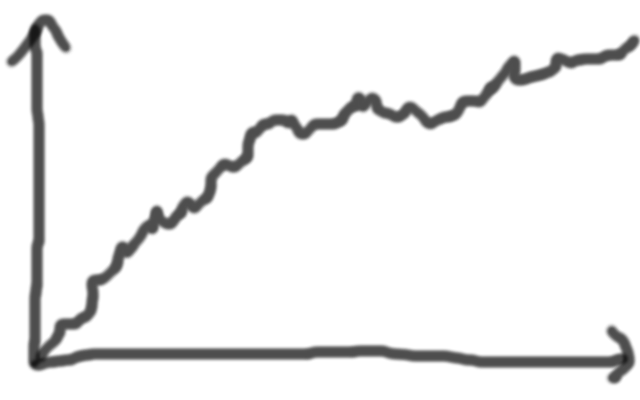
\includegraphics[width=\textwidth]{pictures/safe_learning.png}
\caption{Ok}
\end{subfigure}
\hfill
\begin{subfigure}[t]{0.495\textwidth}
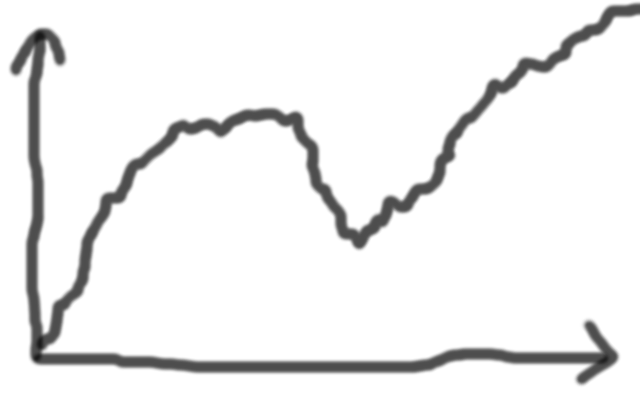
\includegraphics[width=\textwidth]{pictures/unsafe_learning.png}
\caption{Not ok}
\end{subfigure}
\end{figure}
\end{frame}

\begin{frame}
\frametitle{Safe Reinforcement Learning}

\begin{block}{Definition}
Given a reference $\underline{J}$ and a confidence level $\delta$, a RL algorithm is \textbf{safe} if it yields a policy with performance lower than $\underline{J}$ with probability at most $\delta$.

\end{block}

\vfill

\centering
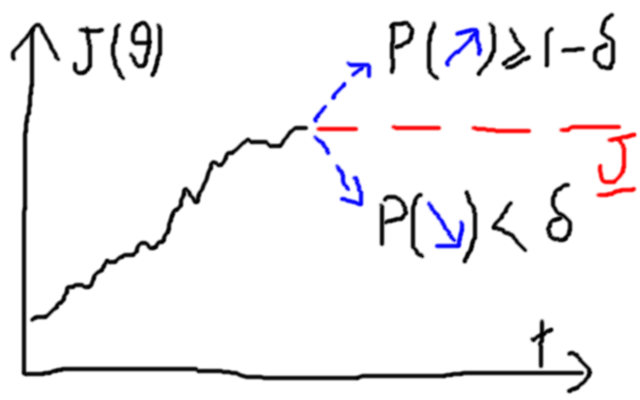
\includegraphics[width=0.48\textwidth]{pictures/safe_explained}


%For instance, monotonic improvement can be defined by a sequence of policies $\pi^0, \pi^1, \ldots, \pi^t$ where $J(\pi^t) \leq J(\pi^{t-1})$ with probability at most $\delta$ for every $t$.

\end{frame}

%%%%%%%%%%%%%%%%%%%%%%%%%%%%%%%%%%%%%%%%%%%%%%%%%%%%%%%%%%%%%%%%%%%%%%%%%%%%%%%%%%%%%%%%%%%%%%%%%%%%%%%%%%%%%%%%%%%%

%\begin{frame}
%\frametitle{Stato dell'arte nell'apprendimento sicuro (1)}
%
%\begin{itemize}
%\item Conservative policy improvement~\cite{kakade}
%\begin{itemize}
%	\item Supponendo $\pi' \gets \alpha \pi + (1 - \alpha)\overline{\pi}$ dove $\overline{\pi}$ corrisponde alla greedy policy,
% $$J(\pi') - J(\pi) \geq \frac{\alpha}{1-\gamma} \left( \mathbb{A}_{\pi}^{\overline{\pi}} - \frac{2\alpha\gamma\epsilon}{1-\gamma(1-\alpha)} \right)$$
%	\item Dunque abbiamo apprendimento sicuro se $\alpha^* = \frac{(1-\gamma)\mathbb{A}_{\pi}^{\overline{\pi}}}{4R}$, dove $R$ è il massimo rinforzo ottenibile.
%\end{itemize}
%
%\item Safe policy iteration~\cite{safe_iteration}
%\begin{itemize}
%\item Risultati simili, ma con un bound più stretto: 
%$$J(\pi') - J(\pi) \geq \frac{\mathbb{A}_{\pi}^{\pi'}}{1-\gamma} - \frac{\gamma}{(1-\gamma)^2}{D_\infty^{\pi, \pi'}}^2 \frac{\norm[\infty]{Q^\pi}}{2}$$
%\end{itemize}
%
%\end{itemize}
%
%
%\end{frame}

%%%%%%%%%%%%%%%%%%%%%%%%%%%%%%%%%%%%%%%%%%%%%%%%%%%%%%%%%%%%%%%%%%%%%%%%%%%%%%%%%%%%%%%%%%%%%%%%%%%%%%%%%%%%%%%%%%%%



\begin{frame}
\frametitle{State of the art in Safe Reinforcement Learning}
We will mainly refer to the results on Adaptive Step Size from~\cite{adaptive_step}

\begin{itemize}
	\item Assuming a policy gradient method with Gaussian-parameterized policies $\pi_{\vtheta}$, an update rule of the form $\vtheta \gets \vtheta + \alpha\gradj$ and \textbf{fixed variance} $\sigma = e^w = const$:
\end{itemize}
\[
J(\vtheta') - J(\vtheta) \geq \textcolor{red}{\alpha} \norm[2]{\nabla_{\vtheta}J(\vtheta)}^2 - \textcolor{red}{\alpha^2} \norm[1]{\nabla_{\vtheta}J(\vtheta)}^2 \frac{c_3 + c_2 \sigma }{c_1 \sigma^3}
\]
\begin{itemize}
	\item that is maximized by the following step size: 
\end{itemize}
	\[
\alpha^* =  \frac{c_1 \textcolor{red}{\sigma^3} \norm[2]{\gradj}^2}{\left(c_2 \textcolor{red}{\sigma} + c_3 \right) \norm[1]{\gradj}^2},
\]
\begin{itemize}
\item that guarantees an improvement of:
\end{itemize}
\[
J(\vtheta') - J(\vtheta) \geq \frac{1}{2}\alpha^* \norm[2]{\gradj}^2.
\]



\end{frame}


\begin{frame}
\frametitle{Problems of Safe Reinforcement Learning}

The results seen so far suffer from the following problems:
\begin{itemize}
\item They target only \textbf{monotonic improvements}
\begin{itemize}
\item This covers only specific user needs.
\end{itemize}
\item They do not consider an \textbf{adaptive variance}
\begin{itemize}
\item The exploration factor remains constant and highly depends on the domain.
\end{itemize}
\item They are \textbf{overly conservative}
\begin{itemize}
\item Resulting in a very slow convergence speed.
\end{itemize}

\end{itemize}


\end{frame}




%%%%%%%%%%%%%%%%%%%%%%%%%%%%%%%%%%%%%%%%%%%%%%%%%%%%%%%%%%%%%%%%%%%%%%%%%%%%%%%%%%%%%%%%%%%%%%%%%%%%%%%%%%%%%%%%%%%
\section{The role of exploration}

\begin{frame}
\frametitle{Exploration in Reinforcement Learning}
\centering
%\includegraphics[width=0.7\textwidth]{pictures/mdp_policy2}
\animategraphics[autoplay,loop,width=0.9\linewidth]{24}{pictures/mountain_car_animation4}{}{}
\end{frame}


\begin{frame}
\frametitle{Exploration in Reinforcement Learning}
Exploration is intended as performing actions that are \textbf{different} than the ones the agent is used to.

\begin{itemize}
\addtolength{\itemsep}{.2cm}
\item Obtain more informations about the environment
\item Find new solutions (possibly better)
\item Escape from local maxima
\end{itemize}

\end{frame}



%%%%%%%%%%%%%%%%%%%%%%%%%%%%%%%%%%%%%%%%%%%%%%%%%%%%%%%%%%%%%%%%%%%%%%%%%%%%%%%%%%%%%%%%%%%%%%%%%%%%%%%%%%%%%%%%%%%%



%%%%%%%%%%%%%%%%%%%%%%%%%%%%%%%%%%%%%%%%%%%%%%%%%%%%%%%%%%%%%%%%%%%%%%%%%%%%%%%%%%%%%%%%%%%%%%%%%%%%%%%%%%%%%%%%%%%%%%%%%%%%%%%%%%%%%%%%%%%%%%%%%%%



\section{Safely-Exploring Policy Gradient (SEPG)}

%\begin{frame}
%\frametitle{Motivazione}
%
%I metodi di apprendimento sicuro visti finora hanno le seguenti problematiche:
%\begin{itemize}
%\item Considerano solo \textbf{miglioramenti monotoni}
%\begin{itemize}
%\item Copre solamente esigenze particolari.
%\end{itemize}
%\item Non considerano una \textbf{esplorazione adattiva}
%\begin{itemize}
%\item Il fattore esplorativo rimane costante e dipende dal problema da risolvere.
%\end{itemize}
%\item Sono molto \textbf{conservativi}
%\begin{itemize}
%\item Richiedono tempi di convergenza molto lunghi
%\end{itemize}
%
%\end{itemize}
%
%
%\end{frame}

\begin{frame}
\frametitle{Contributions (1)}
We extended the performance improvement bounds to include an adaptive exploration factor:

\[
J(\vv, w') - J(\vv, w) \geq \beta \nabla_w J(\vv',w)^2 - d \beta^2 \nabla_w J(\vv',w)^2
\]
that is maximized by:
\[
\beta^* = \frac{1}{2d}
\]
which guarantees:
\[
J(\vv, w') - J(\vv, w) \geq \frac{\nabla_w J(\vv',w)^2}{4d}
\]

\framebox{\begin{minipage}{4cm}\textbf{Recall:}\begin{tightcenter} $\vtheta = [ \vv ; w ]$ \end{tightcenter} \end{minipage}}



\end{frame}




\begin{frame}{Contributions (1)}
\begin{tightcenter}
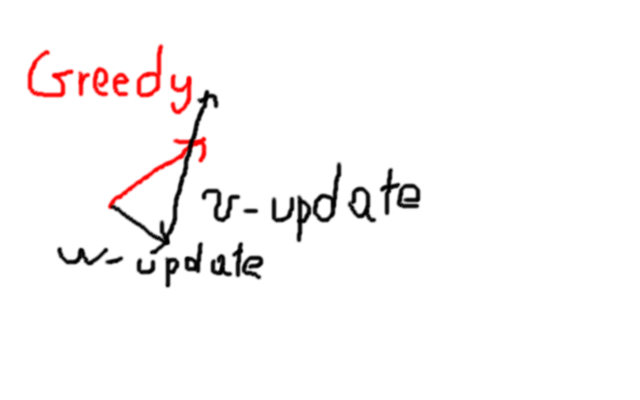
\includegraphics[width=0.4\textwidth]{pictures/newgradient}
\end{tightcenter}

We adapted the results by employing a new gradient direction: 
\[
w \gets w + \beta \gradDelta(\vv, w),
\]
where: 
\[
\gradDelta(\vv, w) := \nabla_w \left( J(\vv', w) - J(\vv, w) \right)
\]
\end{frame}



\begin{frame}{Contributions (1)}
We employed the budget trick to allow for a customizable implementation of this type of update (and more).
\vfill

\centering
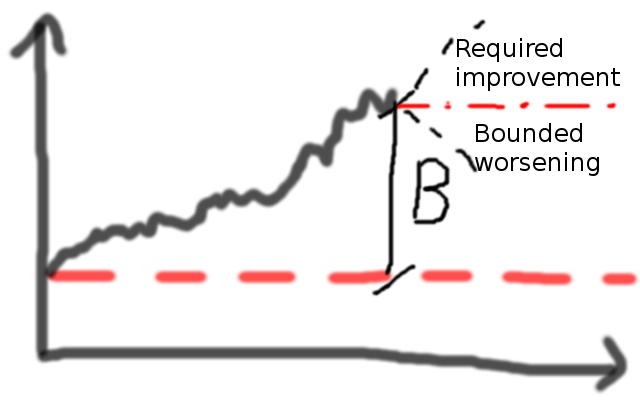
\includegraphics[width=0.6\textwidth]{pictures/budget_image}
\end{frame}




\begin{frame}
\frametitle{Contributions (2)}
The second contribution was to introduce a new framework that goes beyond the single monotonic improvement case.
\vspace{0.3cm}
%\vfill
\begin{columns}[T]
\column{0.5\textwidth}
\centering
\textbf{Type-I}
\vspace{0.3cm}
\begin{itemize}
\item We guarantee $J(\vtheta^t) \geq \jbase$ for each \textbf{policy update}.
\item Suited for systems that requires high reliability.
\end{itemize}
\column{0.5\textwidth}
\centering
\textbf{Type-II}
\vspace{0.3cm}
\begin{itemize}
\item We guarantee $J(\vtheta^t)\geq \jbase$  \textbf{on average} over a learning iteration \\ (\eg a production day).
\item Suited for systems with lower safety needs.
\end{itemize}
\end{columns}

\end{frame}

\begin{frame}
\frametitle{Contributions (2)}
\begin{columns}[T]
\column{0.5\textwidth}
\centering
\textbf{Type-I}

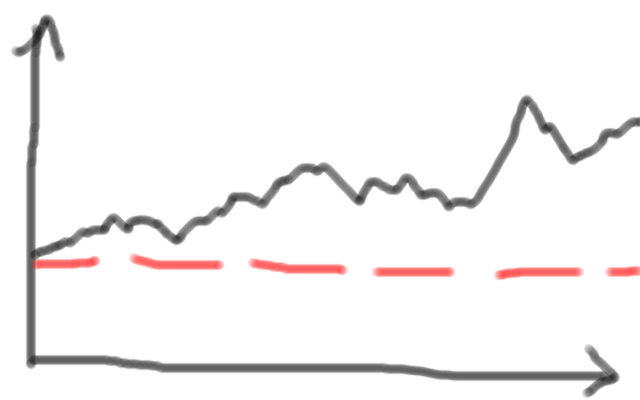
\includegraphics[width=\textwidth]{pictures/plot_safe_1.png}

\column{0.5\textwidth}
\centering
\textbf{Type-II}

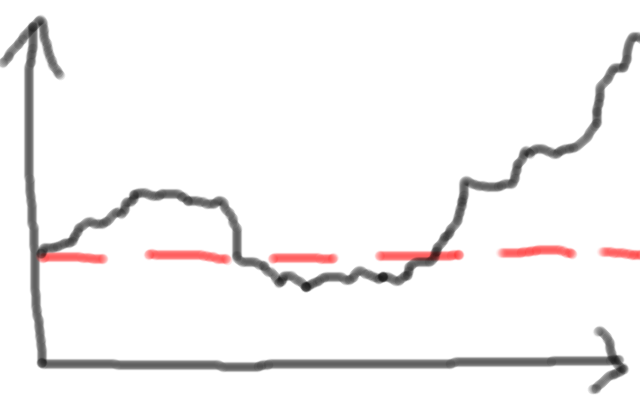
\includegraphics[width=\textwidth]{pictures/plot_safe_2.png}

\end{columns}
\end{frame}


\begin{frame}{Contributions (2)}
In these classes we have identified several variants:
\renewcommand{\arraystretch}{1.6}



\begin{tabular}[t]{R{0.1\textwidth} m{0.85\textwidth}}
\textbf{MI} & Monotonic Improvement with type-I safety \\
\textbf{LB-I} & Lower bounds to the initial policy with type-I safety \\
\textbf{LB-II} & Lower bounds to the initial policy with type-II safety \\
\multicolumn{2}{c}{--- Variants with an additional target policy evaluation ---}\\
\textbf{LV} & A low variance (\eg prototype) policy is tested \\
\textbf{ZV} & The deterministic policy is tested
\end{tabular}

\end{frame}

%%%%%%%%%%%%%%%%%%%%%%%%%%%%%%%%%%%%%%%%%%%%%%%%%%%%%%%%%%%%%%%%%%%%%%%%%%%%%%%%%%%%%%%%%%%%%%%%%%%%%%%%%%%%%%%%%%





\begin{frame}
\frametitle{Contributions (3)}
We devised a new general algorithm that can be customized to specific user needs.

\begin{algorithm}[H]
\caption{Safely-Exploring Policy Gradient}
    \begin{algorithmic}[1] 
	\State \textbf{input:} $\vtheta^0 = [\vv^0, w^0]$, $B^0$
        
%        \State \textbf{evaluate} $\jbase[0] = J(\vv^0, w^0)$
        %\For {t = 1,2 \ldots}
        \State \textbf{for} $t = 1,2\ldots$ \textbf{do}\newline
%        \State\newline
        \hspace*{-\fboxsep}\colorbox{aliceblue}{\parbox{\linewidth}{
            \State \qquad  $\vv^{t+1} \gets \vv^t + \overline{\alpha}\nabla_{\vv}{J(\vv^t, w^t)}$  \Comment{$\vv$-update}
            \State \qquad $B \gets B + J(\vv^{t+1}, w^t) - J(\vv^t, w^t)$.\Comment{$\vv$-budget update}}}
\newline
\hspace*{-\fboxsep}\colorbox{bisque}{\parbox{\linewidth}{
            
            \State \qquad $w^{t+1} \gets w^t + \overline{ \beta}\gradDelta(\vv^{t+1},w^t)$ \Comment{$w$-update}            
            \State \qquad $B \gets B + J(\vv^{t+1}, w^{t+1}) - J(\vv^{t+1}, w^t)$. \Comment{$w$-budget update}}}
%        \EndFor
\State \textbf{end for}
    \end{algorithmic}
\end{algorithm}

\end{frame}

\section{Results}
\begin{frame}
\frametitle{Results - Mountain Car task}
\centering
\begin{figure}
\begin{subfigure}[t]{0.49\textwidth}
\includegraphics[width=\textwidth]{pictures/plot_MC3}
\caption{Evolution of the performance}
\end{subfigure}
\begin{subfigure}[t]{0.49\textwidth}
\includegraphics[width=\textwidth]{pictures/plot_MC_sigma3}
\caption{Evolution of the exploration parameter}
\end{subfigure}
\end{figure}
\end{frame}

%\begin{frame}
%\frametitle{Results - Linear Quadratic Gaussian controller}
%\centering
%%\vspace{-0.5cm}
%\begin{figure}
%\begin{subfigure}[t]{\textwidth}
%\begin{subfigure}[t]{0.45\textwidth}
%\includegraphics[width=\textwidth]{pictures/newplots/newplot1}
%\end{subfigure}
%\hfill
%\begin{subfigure}[t]{0.45\textwidth}
%\includegraphics[width=\textwidth]{pictures/newplots/newplot2}
%\end{subfigure}
%\end{subfigure}
%
%\begin{subfigure}[t]{\textwidth}
%\centering
%\includegraphics[width=0.45\textwidth]{pictures/newplots/newplot3}
%\end{subfigure}
%
%\end{figure}
%\end{frame}

\begin{frame}
\frametitle{Results - Linear Quadratic Gaussian controller}

\vspace{-0.3cm}
\begin{figure}[p]
\begin{subfigure}[p]{0.5\textwidth}
\includegraphics[width=1.2\textwidth]{pictures/newplots/newplot1}
\end{subfigure}
\hfill
\begin{subfigure}[p]{0.45\textwidth}
\begin{subfigure}[t]{\textwidth}
\includegraphics[width=1.05\textwidth]{pictures/newplots/newplot2}
\end{subfigure}
\vfill
\begin{subfigure}[b]{\textwidth}
\vspace{-0.3cm}
\includegraphics[width=1.05\textwidth]{pictures/newplots/newplot3}
\end{subfigure}
\end{subfigure}

\end{figure}
\end{frame}

\section{Conclusions}

\begin{frame}{Conclusions}
In this work we have introduced:
\begin{itemize}
\item A new general framework for safe reinforcement learning
\item An adaptive way to explore the environment
\item A general algorithm that can be customized to the user needs
\end{itemize}
\vfill
Further works can focus on:
\begin{itemize}
\item New methods to adapt exploration using previous knowledge about the environment
\item New ways to invest the budget
\item Extend the result beyond the policy gradient method
\end{itemize}

\end{frame}

\begin{frame}
\frametitle{Conclusions}
\LARGE So many questions... \normalsize

\vfill

\centering
\animategraphics[autoplay,loop,controls,width=0.5\linewidth]{30}{pictures/half_cheetah/half_cheetah-}{0}{200}
\end{frame}

\begin{frame}{Conclusions}
\centering
\LARGE Thank you for your attention\\
\vspace{2cm}
Questions?
\end{frame}

\end{document}

